\section{Sistemi bifase}

Le grandezze estensive specifiche sono la media pesata sulle masse:
\[m = m_\alpha + m_\beta \qquad E = E_\alpha + E_\beta\]
\[e = \frac{m_\alpha}{m}e_\alpha + \frac{m_\beta}{m}e_\beta\]
\[\text{frazione massica:} \quad x_\alpha = \frac{m_\alpha}{m} \quad x_\beta = \frac{m_\beta}{m} \]

Dalla regola di Gibbs il numero di variabili intensive indipendenti per bifase monocomponente è 1, pressione e temperatura non sono indipendenti. Lo stato termodinamico è descritto da una coppia intensiva-estensiva oppure da una coppia estensiva-estensiva.

Per un sistema monocomponente trifase, sempre secondo la regola di Gibbs le variabili intensive indipendenti sono 0, lo stato termodinamico è descritto da una coppia estensiva-estensiva.

\subsection{Stati di aggregazione}
\begin{tabular}{p{2.7cm}p{4.5cm}}
    Liq. sottoraffreddato & Non in procinto di evaporare \\
    Liq. saturo & In procinto di evaporare \\
    Vapore umido & Stato di transizione \\
    Vapore saturo & In procinto di condensazione \\
    Vapore surriscaldato & Non in procinto di condensazione \\
\end{tabular}

\subsection{Diagramma di stato P-v-T}

\begin{center}
    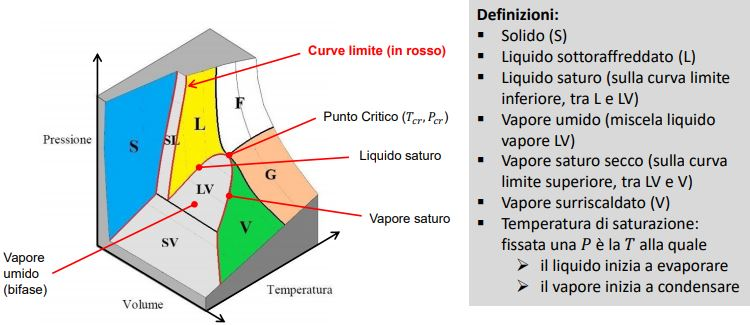
\includegraphics[height=3cm]{Diagramma di stato P-v-T.JPG}
\end{center}


\subsection{Entalpia (calore) di transizione}
La transizione di fase è a P costante: $\dd{h} = \delta q$ (calore necessario = entalpia di transizione).

\[ h_\text{solido} < h_\text{liquido} < h_\text{vapore} \]

Per l'acqua allo stato triplo:
\begin{tabular}{ll}
    Solidificazione & $h_{lst,\ch{H2O}} = \SI{-333}{kJ/Kg}$ \\
    Evaporazione & $h_{lvt,\ch{H2O}} = \SI{2501.6}{kJ/Kg}$
\end{tabular}

\subsection{Titolo di vapore, liquido e solido}
\[ x = x_v = \frac{m_v}{m} \quad x_l = \frac{m_l}{m} \quad x_s = \frac{m_s}{m} \]
\[ x_v + x_l + x_s = 1 \]

Per \textbf{interpolare lineare} nelle tabelle:
\[ Y = Y_A + \frac{Y_B-Y_A}{X_B-X_A}(X-X_A) \]
$Y$: grandezza che si vuole calcolare \newline
$X$: grandezza conosciuta \newline
$A, B$: stati di riferimento (presenti in tabella) con $X_A < X < X_B$ \newline
oppure
\[ \frac{X-X_1}{X_2-X_1} = \frac{T-T_1}{T_2-T_1} \]
\ \newline \newline
Per \textbf{interpolare bilinearmente} nelle tabelle:
\[ Y = Y_A + \frac{Y_B-Y_A}{X_B-X_A}(X-X_A) \]
con
$Y_A = Y_{A1} + \frac{Y_{A2} - Y_{A1}}{X_{A2 - X_{A1}}}(X_A-X_{A1})$
$Y_B = Y_{B1} + \frac{Y_{B2} - Y_{B1}}{X_{B2 - X_{B1}}}(X_B-X_{B1})$

\subsection{Liquidi sottoraffreddati}

Per i liquidi sottoraffreddati non abbiamo le tabelle, ma sappiamo che in generale un liquido sottoraffreddato ha valori approssimabili a quelli del liquido saturo a pari temperatura. Per fare approssimazioni il più precise possibili usiamo il modello di liquido incomprimibile perfetto ($c = $ cost) o anche ideale:
\[
    h(P,T) = h_{ls}(P_{sat}(T)) + v (P - P_{sat}(T))
\]

Per $v$ si può usare il valore del liquido saturo fornito in tabella $v = v_{ls}(P_{sat}(T))$.

Notiamo che il termine $v (P-P_{sat}(T))$ è solitamente piccolo e qualche volta trascurabile (il prof consiglia sempre di calcolarlo).
\newline
Cosa fare se conosciamo $P$ e $h$, ma non $T$? Siccome $v (P-P_{sat}(T))$ è solitamente trascurabile, possiamo dire che $h(P,T) = h_{ls} (P_{sat}(T))$, perciò si interpola in tabella di saturazione la temperatura per la quale $h_{ls} = h$.
[esempio: quale è la temperatura $T$ dell'acqua a $P=80bar$ e $h=1200kj/kg$? notiamo che in questo stato l'acqua è sotto raffreddata, andiamo a cercare quindi nelle tabelle la riga in cui l'entalpia $h$ a liquido saturo è pari a $1200$, e concludiamo che la temperatura è fra i $269,94$ e i $275,56$ gradi, interpolando otteniamo $T=272,96$.]

\subsection{Relazioni semplificate vicino al punto triplo per l'acqua}

In assenza di tabelle, si possono usare le seguenti relazioni semplificate in prossimità del punto triplo:
\begin{itemize}
    \item stato solido: $h(P,T) = \dots$, $s(P,T) = \dots$ (vedi slide)
    \item stato liquido: $h(P,T) = \dots$, $s(P,T) = \dots$ (vedi slide)
    \item stato vapore: $h(P,T) = \dots$, $s(P,T) = \dots$ (vedi slide)
\end{itemize}
Il concetto è che si usa il punto triplo come stato di riferimento, per poi scostarsi da esso per approssimare il dato cercato.